\documentclass{article}

\usepackage[french]{babel}
\usepackage[utf8]{inputenc}
\usepackage{lipsum}
\usepackage{amsmath, amssymb, amsthm, graphicx}
\usepackage{tikz}
\usepackage{cite}
\usepackage{multicol}
\usepackage[hidelinks]{hyperref}
\usepackage{caption}
\captionsetup{font=footnotesize}
\usepackage{multirow}
\usepackage{adjustbox}
\usepackage{listings}
\usepackage{float}
\setlength{\parindent}{0pt}
\newtheorem{theorem}{Théorème}
\graphicspath{{./img}}

%%%%%%%%%%%%%%%% Lengths %%%%%%%%%%%%%%%%
\setlength{\textwidth}{16.5cm}
\setlength{\evensidemargin}{-0.5cm}
\setlength{\oddsidemargin}{-0.5cm}
\setlength{\topmargin}{-1.5cm}
\setlength{\textheight}{23cm}


%%%%%%%%%%%%%%%% Variables %%%%%%%%%%%%%%%%
\def\projet{4}
\def\titre{Systèmes non linéaires}
\def\groupe{4}
\def\equipe{4}
\def\responsible{Numa Guiot}
\def\secretary{Sohayb El Yaktini}
\def\others{Melissa Colin, Mohamed Ajaji}

\begin{document}

%%%%%%%%%%%%%%%% Header %%%%%%%%%%%%%%%%
\begin{minipage}{0.98\textwidth}
  \vskip 0mm
    { \begin{tabular}{p{7.5cm}}
      {\bfseries \sffamily
        Projet \projet} \\ 
      {\itshape \titre}
    \end{tabular}}
  \hfill 
  \fbox{\begin{tabular}{l}
      {~\hfill \bfseries \sffamily Groupe \groupe\ - Équipe \equipe
        \hfill~} \\[2mm] 
      Responsable : \responsible \\
      Secrétaire : \secretary \\
      Codeurs : \others
    \end{tabular}}
  \vskip 4mm ~

  ~~~\parbox{0.95\textwidth}{\small \textit{Résumé~:} \sffamily Ce travail présente la méthode de Newton-Raphson pour résoudre des systèmes d'équations non linéaires. Nous avons implémenté cette méthode et l'avons appliquée à deux cas d'utilisation : la recherche d'équilibre avec les points de Lagrange et la méthode de Bairstow pour trouver les racines complexes d'un polynôme.}
  \vskip 1mm ~
\end{minipage}

%%%%%%%%%%%%%%%%% TEMPLATE %%%%%%%%%%%%%%%%
\section{Introduction}
Courte pharse ici

\subsection{Contexte}
La résolution de systèmes d'équations non linéaires est un problème fondamental en mathématiques appliquées et en ingénierie. Ces systèmes apparaissent dans de nombreux domaines, tels que la physique, la chimie, l'économie et l'informatique. La recherche de solutions à ces systèmes est souvent complexe et nécessite des méthodes numériques efficaces. Dans ce projet, nous allons nous intéresser à la méthode de Newton-Raphson, qui est une méthode itérative largement utilisée pour résoudre des systèmes d'équations non linéaires. Nous allons également explorer deux applications de cette méthode : la recherche d'équilibre dans un système de deux masses en interaction gravitationnelle et la méthode de Bairstow pour trouver les racines complexes d'un polynôme.

\subsection{Motivation}
La motivation de ce projet est de comprendre et d'implémenter la méthode de Newton-Raphson pour résoudre des systèmes d'équations non linéaires. Nous allons également explorer deux applications de cette méthode : la recherche d'équilibre dans un système de deux masses en interaction gravitationnelle et la méthode de Bairstow pour trouver les racines complexes d'un polynôme. Ces applications nous permettront de mettre en pratique la méthode de Newton-Raphson et de mieux comprendre son fonctionnement ainsi que ses faiblesses.

\section{Méthodologie}
Dans ce travail,  nous avons implémenter la méthode de Newton-Raphson afin de résoudre des systèmes d'équations non linéaires. Pour éprouver notre méthode, nous avons choisi de résoudre deux problèmes différents. Le premier, consiste à trouver les positions d'équilibre d'un système de deux masses en interaction gravitationnelle, en utilisant les points de Lagrange. Le second à pour objectif de trouver les racines complexes d'un polynôme avec la méthode de Bairstow. Nous avons donc aussi implémenté ces deux méthodes. \\ \\
L'ensemble des expérimentations a été réalisé sur un système avec un processeur AMD Ryzen 7 7840HS et 64 Go de RAM. %et une carte graphique NVIDIA RTX A500 Laptop GPU.

\subsection{Méthode de Newton-Raphson}
\label{sec:methodo}
La méthode de Newton-Raphson est une méthode itérative qui permet de trouver les zéros d'une fonction. \\ \\
Soit \(f\) la fonction dont on cherche les racines et \(H\) sa matrice jacobienne. On détermine \(U\), un vecteur initial, qui nous permet de calculer \(f(U)\) et \(H(U)\). \\
On cherche alors ensuite un vecteur \(V\) tel que \(f(U+V) = 0\). Nous pouvons approximer \(f(U+V)\) par \(f(U) + H(U)V\). Nous cherchons alors la solution au système linéaire \(f(U)+H(U)V = 0\), autrement dit \textcolor{red}{\(H(U)V = -f(U)\)}.\\
On peut alors utiliser une décomposition QR pour résoudre ce système, ce qui nous donne \(H(U) = QR\) et \(RV = -{}^{t}Qf(U)\), étant donné \(Q\) orthogonale.\\
On résout ainsi ce système linéaire en utilisant \texttt{np.linalg.lstsq(R, -np.dot(Q.T, f(U)))} pour trouver \(V\) et éviter les problèmes numériques pour les matrices dont le déterminant est presque nul.\\
On a donc \(U = U + V\) et on réitère jusqu'à ce que la norme de \(V\) soit inférieure à une certaine tolérance. \\ \\
Pour améliorer la convergence de la méthode, nous avons rajouté un backtracking qui vérifie si la norme de \(f(U + \alpha V)\) est plus petite que la norme de \(f(U)\).\\
Pour ce faire, on commence par choisir un pas \texttt{$\alpha$} et on calcule \texttt{f(U + $\alpha$V)}.
Si \(||f(U + \alpha V)||\) est plus petit que \(||f(U)||\), on a trouvé un meilleur point et on continue avec ce point.
Sinon, on réduit \(\alpha\) et on réitère jusqu'à trouver un point qui minimise \(||f(U + \alpha V)||\). \\ \\

Pour visualiser la convergence de cette méthode, nous avons réalisé un premier graphique qui permet de visualiser l'évolution de la norme de \(f(U)\) en fonction du nombre d'itérations avec et sans backtracking en prenant \(f(x)=x^2-2\) et \(U_0 = 0.001\). 
Nous avons ensuite réalisé deux graphiques permettant de comparer le temps de convergence (en secondes) et la précision du résultat selon la taille de la matrice d'entrée pour nos deux méthodes avec et sans backtracking ainsi que la méthode de \texttt{np.linalg.solve}. Pour ce faire, nous itérons 20 fois sur des matrices aléatoires de taille \(n \in [2, 100]\) et nous calculons la moyenne des temps de convergence et des erreurs. Nous initialisons \(U_0\) avec des valeurs aléatoires et si celles-ci ne donnent pas de résultats, nous tentons plusieurs fois d'en trouver une qui fonctionne.

\subsection{Recherche d'équilibre avec les points de Lagrange}
\label{sec:lagrange}
Nous avons ensuite utilisé la méthode de Newton-Raphson pour trouver les points d'équilibre d'un système de deux masses en interaction gravitationnelle. Les points de Lagrange sont des points dans l'espace où la somme des forces gravitationnelles et centrifuges est nulle. Nous allons utiliser ces points pour trouver les positions d'équilibre du système. \\ \\
Considérant les vecteurs de coordonnées \((x, y)\) pos1 et pos2 de deux objets et leurs masses \(k1\) et \(k2\) respectivement, nous pouvons obtenir leur barycentre par \(B = \frac{k1 \cdot \text{pos1} + k2 \cdot \text{pos2}}{k1 + k2}\). Nous pouvons alors, à partir de celui-ci et \(kc\), sa masse, déterminer la force centrifuge exercée sur un objet de position \(U\) par \(F_c = kc(U - \text{B})\). \\
Nous pouvons alors calculer la force gravitationnelle exercée sur \(U\) par chacune des masses en utilisant la loi de Newton qui nous donne \(F_g = \frac{-k \cdot (U - \text{pos})}{||U - \text{pos}||³}\). \\ 

Ainsi, nous cherchons à déterminer la position d'équilibre \(U\) telle que la somme des forces gravitationnelles et centrifuges soit nulle. Nous appliquons alors la méthode de Newton-Raphson à notre système somme des forces à partir de la position \(U = [1.5,0]\) telle que fournie par le sujet. \\ \\

Nous avons ensuite visualisé les points d'équilibre "points de Lagrange" en appliquant la méthode de Newton-Raphson sur 5 vecteurs \(U_x\) correspondant à notre vecteur \(U\) précédent plus ou moins 5 sur chaque axe. Nous avons ensuite calculé la force totale exercée sur chaque point \(U\) et nous avons visualisé la magnitude de cette force afin de la représenter sous forme de carte de chaleur. Nous avons ensuite superposé les points d'équilibre sur cette carte de chaleur afin de visualiser les zones d'équilibre.

\subsection{Méthode de Bairstow pour les polynômes}
Newton-Raphson est une méthode efficace pour trouver les racines d'un polynôme, mais elle ne fonctionne que pour des racines réelles. Pour les polynômes dont les racines sont complexes, nous devons utiliser une méthode différente. La méthode de Bairstow est une méthode itérative qui permet de trouver les racines d'un polynôme en utilisant la méthode de Newton-Raphson. Elle est particulièrement utile pour les polynômes de degré supérieur à 2, car elle permet de trouver les racines complexes en utilisant des coefficients réels. \\ \\
Pour cette méthode nous suivrons les résultats présentés dans \textit{Numerical Recipes in C}\\
Soit \(P(x)\) un polynôme de degré \(n\). Nous cherchons alors un facteur quadratique de la forme \(x^2 + Bx + C\) qui divise \(P(x)\), c'est à dire tel que \(P(x) = (x^2 + Bx + C)Q(x) +Rx + S\), où \(Q(x)\) est un polynôme de degré \(n-2\) et \(R\) et \(S\) des constantes, reste de la division.\\

Nous cherchons alors à déterminer \(B\) et \(C\) pour la fonction \(F(B,C) = (R,S)\) tel que \(F(B,C) = 0\) pour ainsi annuler le reste \(Rx + S\) de la division.\\ Le domaine de définition de cette fonction est l'ensemble des couples \((B, C)\) de nombres réels.\\
Ces valeurs correspondent sont celles qui font que \(x^2 + Bx + C\) est un facteur de \(P(x)\).\\ \\
Pour appliquer Newton-Raphson à ce système, nous devons d'abord calculer la matrice jacobienne \(J\) de \(F\). Pour calculer ces dérivées partielles de R et S par rapport à B et C on à \(\frac{\partial R}{\partial B} = BR_1 - S_1\), \(\frac{\partial R}{\partial C} = -R_1\), \(\frac{\partial S}{\partial B} = CR_1\) et \(\frac{\partial S}{\partial C} = -S_1\) où \(R_1\) et \(S_1\) sont les restes de la division de \(Q(x)\) par le facteur quadratique \(x^2 + Bx + C\). La matrice jacobienne $J$ est donc donnée par l'équation suivante : 
\begin{equation}
J = \begin{bmatrix}
\frac{\partial R}{\partial B} & \frac{\partial R}{\partial C} \\
\frac{\partial S}{\partial B} & \frac{\partial S}{\partial C}
\end{bmatrix}
=
\begin{bmatrix}
BR_1 - S_1 & -R_1 \\
CR_1 & -S_1
\end{bmatrix}
\label{eq:jacobian}
\end{equation}

Cette matrice jacobienne est utilisée dans l'algorithme de Newton-Raphson pour trouver les valeurs de $B$ et $C$ qui annulent le reste $Rx + S$ de la division. Ainsi nous trouverons certaines racines de \(P(x)\) en résolvant celles du sytsème quadratique : \(P(x) = (x^2 + Bx + C)\).\\ \\ 

% Nous avons aussi tracé la fonction \(F(B,C)\) pour visualiser les points de convergence de la méthode de Bairstow. Nous avons ensuite comparé les résultats obtenus avec ceux de la méthode de Newton-Raphson et ceux de la méthode de Bairstow. \\ \\
\section{Résultats et discussions}
Dans cette section, nous présenterons les résutats quant à l'implémentation de la méthode de Newton-Raphson, la recherche d'équilibre avec les points de Lagrange et la méthode de Bairstow pour les polynômes.

\subsection{Méthode de Newton-Raphson}
La figure~\ref{fig:Newton-Raphson} représente l'évolution de la norme de \texttt{f(U)} en utilisant la méthode de Newton-Raphson en fonction du nombre d'itérations avec et sans backtracking sur l'exemple \texttt{f(x) = x² - 2} et \texttt{$U_{0}$ = 0.001}. Celle-ci met en évidence la différence entre l'utilisation ou non de backtracking. En effet, sans backtracking, il est possible d'avoir des "sauts" comme on le voit sur la première itération : c'est-à-dire que d'une itération à l'autre, la norme de \texttt{f(U)} peut augmenter. Nous pouvons aussi observer que la convergence passe de linéaire à quadratique au niveau de la douzième itération sans utilisation de backtracking alors qu'avec backtracking, c'est au niveau de la deuxième itération (bien que sur cet exemple, la convergence soit rapide en général). L'utilisation de backtracking permet donc une convergence en moins d'itérations et plus stable. 
\begin{figure}[H]
  \centering
  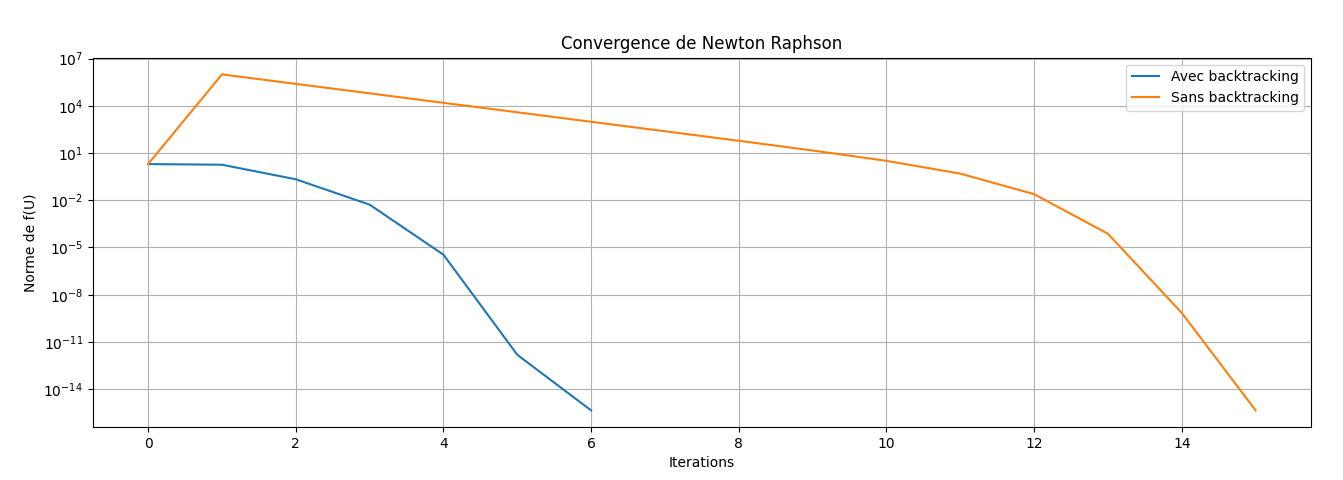
\includegraphics[width=1\textwidth]{convergence_comparison.png}
  \caption{Évolution de la norme de \texttt{f(U)} en fonction du nombre d'itérations avec et sans backtracking}
  \label{fig:Newton-Raphson}
\end{figure}
Bien que le nombre d'itérations soit plus faible avec le backtracking, le temps pour chaque itération est plus long. En effet, le backtracking nécessite de calculer la norme de \texttt{f(U + $\alpha$V)} pour chaque itération, ce qui est plus coûteux que de simplement calculer \texttt{f(U)}. Cependant, le temps total de convergence est plus faible avec le backtracking quand la solution nécessite un grand nombre d'itérations. \\
Ainsi, la figure~\ref{fig:performance-Newton-Raphson} permet non seulement d'observer cette différence en temps qui semble très faible entre nos deux méthodes mais aussi de comparer notre implémentation de Newton-Raphson avec la méthode \texttt{Numpy} qui utilise la méthode de Gauss pour résoudre le système linéaire. 
\begin{figure}[H]
  \centering
  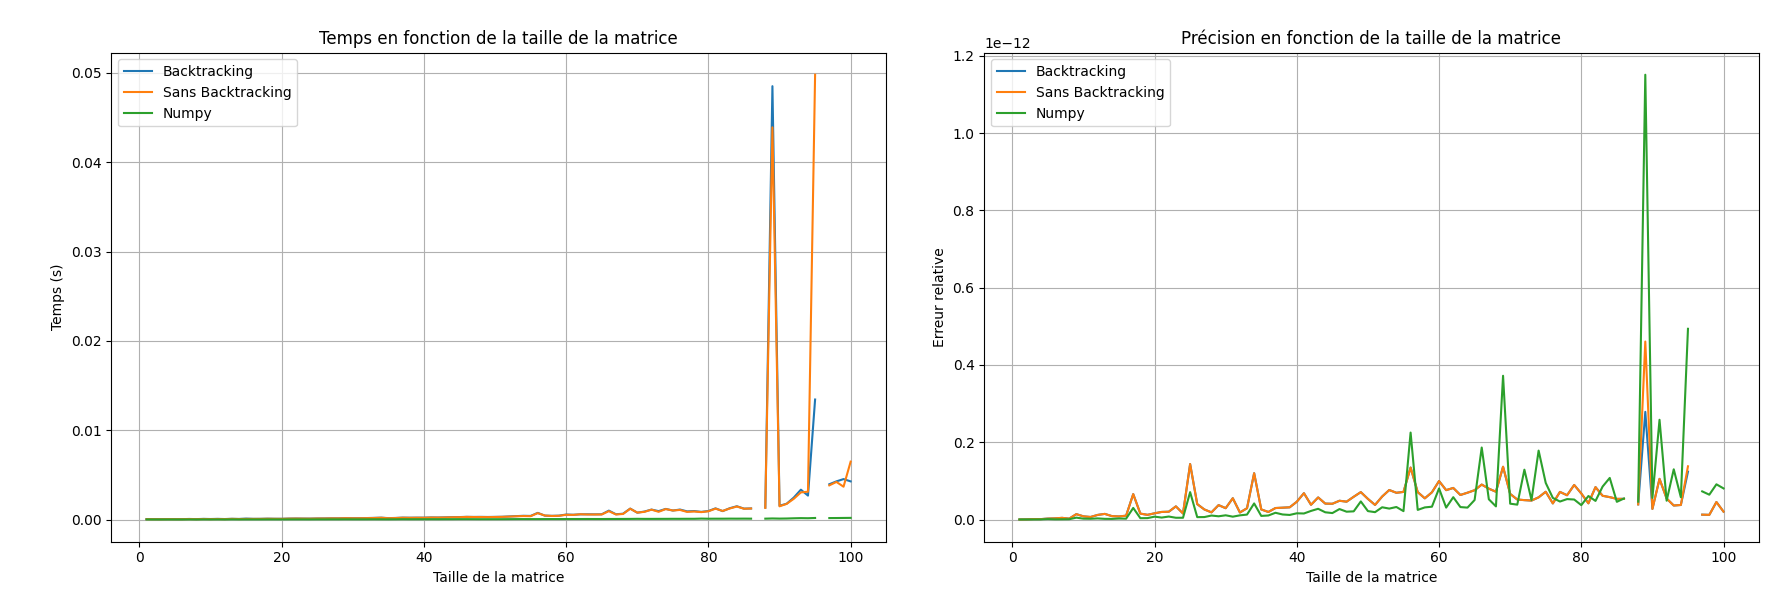
\includegraphics[width=1.1\textwidth]{time_and_precision_vs_size.png}
  \caption{Temps de convergence et précision en fonction de la taille de la matrice}
  \label{fig:performance-Newton-Raphson}
\end{figure}
Nous pouvons observer plusieurs manques sur les deux graphiques, ceux-ci sont dus à l'échec de convergence répété sur certaines tailles de matrices. On observe aussi plusieurs sauts qui se produisent aux mêmes moments sur le temps et l'erreur pour l'ensemble des méthodes, ceux-ci représentent une très grande difficulté à converger due à une valeur de départ très éloignée. Il semblerait que dans ces cas-ci, notre méthode soit généralement plus précise que celle de numpy, surtout celle avec backtracking (par exemple sur la 90ème itération), ce qui s'explique notamment par le fait que numpy privilégie la vitesse à la précision, on observe effectivement une résolution en temps constant indépendamment de la taille de la matrice.

\subsection{Recherche d'équilibre avec les points de Lagrange}
L'utilisation de la méthode de Newton-Raphson pour trouver les points d'équilibre du système de deux masses en interaction gravitationnelle a été un succès. 

\begin{figure}[H]
  \centering
  \begin{minipage}{0.45\textwidth}
  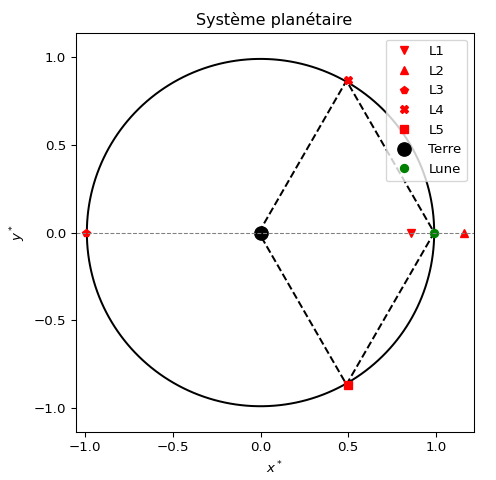
\includegraphics[width=\textwidth]{syteme_planaire.png}
  \caption{Système de deux masses en interaction gravitationnelle}
  \label{fig:lagrange-points}
  \end{minipage}%
  \hfill
  \begin{minipage}{0.5\textwidth}
  Nous avons pu trouver les positions d'équilibre du système et vérifier que nous obtenions bien les valeurs fournies. Nous avons ensuite utilisé ces points pour visualiser les zones d'équilibre du système.\\ \phantom{text} \\
  La figure~\ref{fig:lagrange-points} illustre les cinq points de Lagrange pour le système présenté en section \ref{sec:lagrange} (nous avons représenté les deux masses comme Terre et Lune). Cette représentation permet de confirmer visuellement que les points de Lagrange sont bien des points d'équilibre du système. Cette conclusion est encore plus flagrante avec la graphique suivant.
  \end{minipage}
\end{figure}


\begin{figure}[H]
  \centering
  \begin{minipage}{0.5\textwidth}
  Pour mieux visualiser ces points par rapport à la force totale exercée sur l'objet, nous avons aussi représenté la magnitude de la force totale exercée sur l'objet à différentes positions de l'espace pour visualiser les zones d'équilibre. Nous avons ensuite superposé les points de Lagrange sur cette carte de chaleur. La figure~\ref{fig:lagrange-heat} illustre cette carte de chaleur. Nous pouvons alors facilement visualiser que la force totale est plus faible aux points de Lagrange qu'aux autres positions, ce qui confirme que ces points sont bien des points d'équilibre du système. De plus, on peut observer que la force totale est plus forte près des deux masses, ce qui est logique puisque celles-ci exercent une force gravitationnelle sur l'objet.
  \end{minipage}
  \hfill
  \begin{minipage}{0.45\textwidth}
  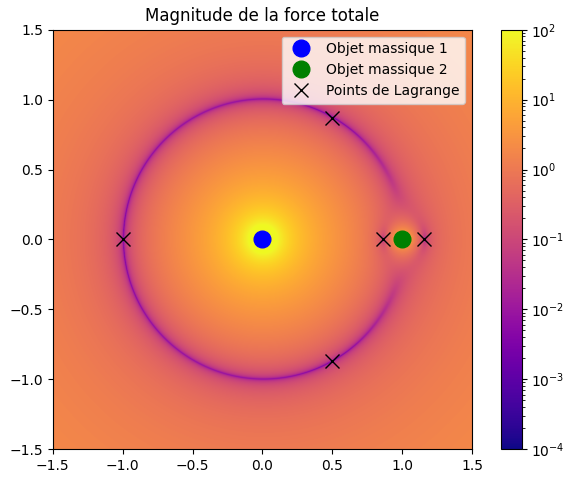
\includegraphics[width=\textwidth]{magnitude.png}
  \caption{Carte de chaleur des forces totales exercées sur l'objet}
  \label{fig:lagrange-heat}
  \end{minipage}%
\end{figure}


\subsection{Méthode de Bairstow pour les polynômes}
La méthode de Bairstow a été appliquée avec succès pour trouver les racines d'un polynôme de degré 3. Nous avons pu trouver les racines du polynôme \(P(x) = x^3 - 6x^2 + 11x - 6\) qui sont \(1, 2, 3\). Nous avons ensuite comparé les résultats obtenus avec ceux de la méthode de Newton-Raphson et ceux de la méthode de Bairstow. Il existe plusieurs méthodes pour choisir les valeurs initiales de B et C. Nous avons utilisé deux méthodes différentes. La première consiste à se baser sur une connaissance préalable des racines du polynôme. En effet si on connaît \texttt{\(r_1\) et \(r_2\)}, deux racines du polynôme, on peut choisir \(B = -(r_1+r_2)\) et \(C = r_1r_2\). Ainsi on peut commencer par prendre \(B = -(1+2)= -3\) et \(C = 1*2 = 2\). Sur cet exemple, on trouve immédiatement les valeurs recherchées. La seconde méthode est utilisée si on ne connait pas les valeurs des racines au préalable. Ainsi, pour un polynome \(P(x) = a_n x^n + a_{n-1} x^{n-1} + ... + a_0\), on choisit \(B = -\frac{a_{n-1}}{a_n} = \frac{6}{1} = 6\) et \(C = \frac{a_0}{a_n} = -\frac{6}{1} = -6\). On itère à partir de ces valeurs pour trouver les racines du polynôme.\\ \\
\begin{figure}[H]
  \centering
  \begin{minipage}{0.56\textwidth}
  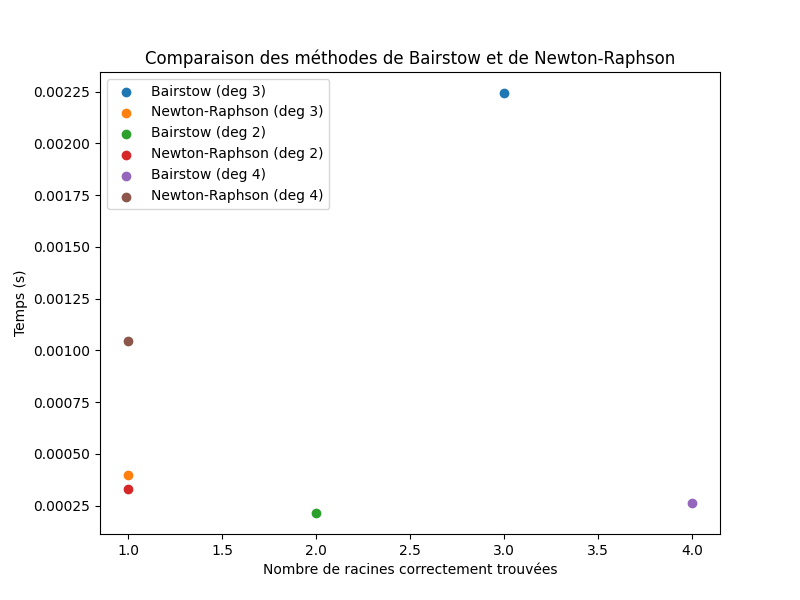
\includegraphics[width=\textwidth]{bairstow_plot.png}
  \caption{Temps de convergence en fonction du nombre de racines trouvées pour chaque méthode sur différents degrés de polynômes}
  \label{fig:bairstow}
  \end{minipage}%
  \hfill
  \begin{minipage}{0.4\textwidth}
  La figure~\ref{fig:bairstow} illustre cette comparaison. Nous pouvons observer que la méthode de Bairstow permet de trouver correctement plus de racines que la méthode de Newton-Raphson ce qui s'explique par le fait que la méthode de Bairstow est plus adaptée pour trouver les racines complexes. Bien que celle-ci ne soit pas nécessairement plus rapide que la méthode de Newton-Raphson, elle est plus robuste et permet de trouver des racines complexes. 
  \end{minipage}%
\end{figure}

\begin{figure}[H]
  \centering
  \begin{minipage}{0.45\textwidth}
  Nous avons ensuite visualisé les résultats obtenus en traçant le polynôme et ses racines pour confirmer graphiquement que les racines trouvées étaient correctes. La figure~\ref{fig:bairstow-plot} illustre cette comparaison. Nous pouvons observer que les racines trouvées par la méthode de Bairstow sont bien celles du polynôme \(P(x)\) et que la méthode de Bairstow permet de trouver des racines complexes.
  \end{minipage}%
  \hfill
  \begin{minipage}{0.5\textwidth}
  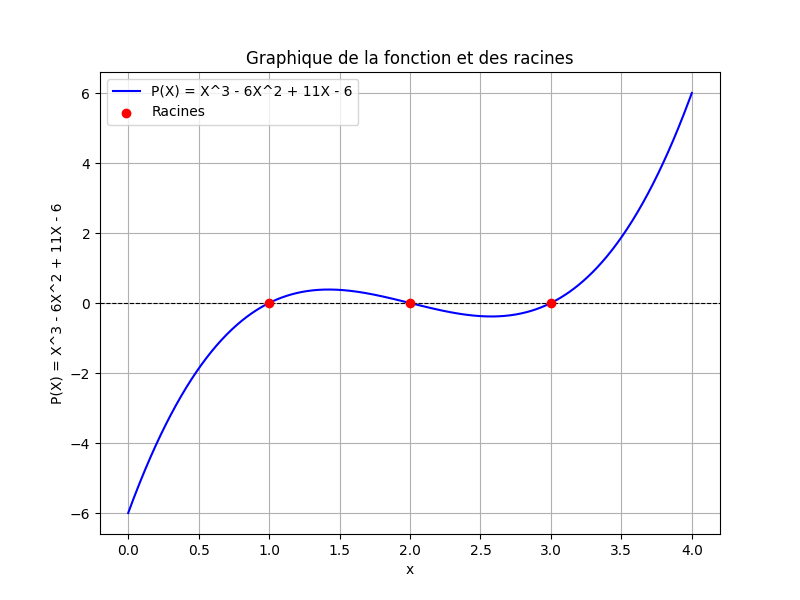
\includegraphics[width=\textwidth]{berstow.png}
  \caption{Visualisation des racines du polynôme \(P(x)\) avec ses racines trouvées par la méthode de Bairstow}
  \label{fig:bairstow-plot}
  \end{minipage}
\end{figure}


\section{Conclusion et perspectives}
En conclusion, ce projet nous a permis de prendre connaissance et d'implémenter la méthode de Newton-Raphson ainsi que de l'appliquer dans deux cas d'utilisation différents : les points de Lagrange et la méthode de factorisation de polynômes de Bairstow. 
\\ \\
Cependant, nous avons rencontré plusieurs problèmes lors de nos expérimentations. Tout d'abord, la méthode de Newton-Raphson est très sensible au choix des conditions initiales. Une mauvaise estimation initiale peut entraîner une divergence ou une convergence lente, comme observé dans certains cas où la solution nécessitait un grand nombre d'itérations. De plus, la méthode peut échouer lorsque la matrice jacobienne est mal conditionnée ou singulière, ce qui a nécessité l'utilisation de techniques comme la décomposition QR pour améliorer la stabilité numérique.
\\ \\
Malgré ces défis, l'utilisation de la méthode de Newton-Raphson présente de nombreux avantages. Elle offre une convergence quadratique lorsque les conditions initiales sont bien choisies, ce qui la rend très efficace pour des problèmes bien posés. L'ajout du backtracking a également permis d'améliorer la robustesse de la méthode, en évitant les "sauts" et en garantissant une diminution monotone de la norme de la fonction.
\\ \\
En comparant nos résultats avec ceux présentés dans le chapitre 9 de \textit{Numerical Recipes}, nous avons constaté que la méthode de Bairstow, bien qu'un peu plus complexe à implémenter, est particulièrement adaptée pour trouver les racines complexes des polynômes. Elle complète efficacement la méthode de Newton-Raphson, qui est mieux adaptée pour des systèmes non linéaires généraux.

\end{document}